%%%%%%%%%%%%%%%%%%%%%%%%%%%%%%%%%%%%%%%%%
% a0poster Portrait Poster
% LaTeX Template
% Version 1.0 (22/06/13)
%
% The a0poster class was created by:
% Gerlinde Kettl and Matthias Weiser (tex@kettl.de)
% 
% This template has been downloaded from:
% http://www.LaTeXTemplates.com
%
% License:
% CC BY-NC-SA 3.0 (http://creativecommons.org/licenses/by-nc-sa/3.0/)
%
%%%%%%%%%%%%%%%%%%%%%%%%%%%%%%%%%%%%%%%%%

%----------------------------------------------------------------------------------------
%	PACKAGES AND OTHER DOCUMENT CONFIGURATIONS
%----------------------------------------------------------------------------------------

\documentclass[a0,portrait]{a0poster}


\usepackage{multicol} % This is so we can have multiple columns of text side-by-side
\columnsep=40pt % This is the amount of white space between the columns in the poster
\columnseprule=3pt % This is the thickness of the black line between the columns in the poster

\usepackage[svgnames]{xcolor} % Specify colors by their 'svg names', for a full list of all colors available see here: http://www.latextemplates.com/svgnames-colors

\usepackage{times} % Use the times font
%\usepackage{palatino} % Uncomment to use the Palatino font

\usepackage{graphicx} % Required for including images
\graphicspath{{figures/}} % Location of the graphics files
\usepackage{booktabs} % Top and bottom rules for table
\usepackage[font=small,labelfont=bf]{caption} % Required for specifying captions to tables and figures
\usepackage{amsfonts, amsmath, amsthm, amssymb} % For math fonts, symbols and environments
\usepackage{wrapfig} % Allows wrapping text around tables and figures
\usepackage[spanish]{babel}



\begin{document}
\renewcommand\abstractname{\Large{}}
%----------------------------------------------------------------------------------------
%	POSTER HEADER 
%----------------------------------------------------------------------------------------

% The header is divided into two boxes:
% The first is 75% wide and houses the title, subtitle, names, university/organization and contact information
% The second is 25% wide and houses a logo for your university/organization or a photo of you
% The widths of these boxes can be easily edited to accommodate your content as you see fit
   
\begin{minipage}[ht]{0.20\linewidth}
    
\includegraphics[width=8cm]{Escudo_UACH.png}\\
\end{minipage}
\begin{minipage}[ht]{0.67\linewidth}
\veryHuge \color{NavyBlue} \textbf{} \color{Black}\\ % Title
\Huge\textit{\color{NavyBlue} Medición de Multímetros en Campos no Conservativos}\\[2cm] % Subtitle
\huge \textbf{Universidad Autónoma de Chihuahua}\\[0.4cm] % University/organization
\Large \texttt Daniel Carrete Guzmán$^{1}$, Jesús Camacho Macías$^{2}$, Edwin Pérez Rodríguez$^{3}$\\[0.3cm] % Author(s)
\texttt{$^{1}$a348564@uach.mx, $^{2}$a348674@uach.mx, $^{3}$a348643@uach.mx \\}
\end{minipage}
\begin{minipage}[ht]{0.15\linewidth}
    
\includegraphics[width=8.5cm]{figures/logo ingenieria.png}\\
\end{minipage}


%----------------------------------------------------------------------------------------

%----------------------------------------------------------------------------------------
%	ABSTRACT
%----------------------------------------------------------------------------------------

\begin{center}
    \begin{minipage}{0.7\textwidth}
        \begin{abstract}
       \centering \section*{Resumen}
       \large
            En este trabajo se obtuvieron resultados experimentales donde se muestran lecturas distintas de medición de $"voltaje"$ en los mismos puntos a consecuencia de un campo inducido, se muestra cómo dichos campos son no conservativos, los cuales por consecuencia hacen que el trabajo realizado dependa de la trayectoria que sigan. Además, esto quiere decir que no pueden tener un potencial independiente de tal campo, entonces ¿qué es lo que medimos? Y ¿Serán las lecturas en ambos multímetros iguales?
        \end{abstract}
    \end{minipage}
\end{center}

% This is how many columns your poster will be broken into, a portrait poster is generally split into 2 columns
\begin{multicols}{2}


%----------------------------------------------------------------------------------------
%	INTRODUCTION
%----------------------------------------------------------------------------------------

\color{black} % SaddleBrown color for the introduction

\section*{Introducción}
\noindent Al colocar una espira cerrada de una sola vuelta cerca de un solenoide por el cual circula una corriente que varía con el tiempo, se induce un campo eléctrico en la espira debido a la variación del flujo magnético a través de ella. Este campo eléctrico puede generar una corriente eléctrica si hay un camino cerrado para el flujo de cargas eléctricas.

\noindent Imaginemos que el solenoide es muy largo y digamos que solamente hay campo magnético dentro de este mismo. Para hacer aproximaciones consideremos el solenoide ortogonal al plano del papel, y también diremos que el flujo magnético es una función lineal del tiempo

\begin{equation}
\boldsymbol{\Phi}=\alpha t,
\label{flujo}
\end{equation}
\noindent donde $\alpha$ es una constante positiva, y una vez establecido esto consideremos el siguiente circuito donde colocamos dos resistencias $R_1$  y $R_2$, de manera simétrica como se muestra en la figura.

\begin{center}\vspace{0.4cm}
    \includegraphics[scale=0.9]{Presentación1.jpg}
    \captionof{figure}{Representación con vista vertical del circuito a analizar}
\end{center}\vspace{0.4cm}
Podemos notar dos nodos A y B, conectados a $M_{1}$ y $M_{2}$ que son los multímetros, es decir, donde se medirán los "potenciales"(palabra que debe de ser definida con cuidado en casos como este). A primera instancia podría resultar intuitivo que al estar midiendo entre ambos nodos A y B los multímetros mostrarán lecturas iguales, pero como  mostraremos más adelante que esto no sucede así para campos inducidos lo cual da como consecuencia lecturas distintas en $M_{1}$y $M_{2}$.

%----------------------------------------------------------------------------------------
%	OBJECTIVES
%----------------------------------------------------------------------------------------

\color{Black} % DarkSlateGray color for the rest of the content

\section*{Cálculos Teóricos}

%----------------------------------------------------------------------------------------
%	Cálculos Teóricos
%----------------------------------------------------------------------------------------
\noindent Antes de continuar es pertinente recalcar algunas distinciones que hace Romer \textbf{[{1}]} en su publicación original.
Consideremos la siguiente integral
\begin{equation}
    \oint_{C_n} \mathbf{E} \cdot d\mathbf{r}.
\end{equation}
Donde $C_n$ son los posibles contornos, tomaremos a $C_R$  como el contorno cerrado de la espira con las resistencias; $C_1$  como el contorno cerrado en sentido antihorario que va del nodo A, atraviesa el multímetro $M_1$ y regresa al nodo A por $R_1$; $C_2$  como el contorno cerrado en sentido horario que va del nodo B, atraviesa el multímetro $M_2$ y regresa al nodo B por $R_2$.



\noindent Tomando en cuenta la ley de Faraday 
\begin{equation}
    \oint_{C_n}  \mathbf{E} \cdot d\mathbf{r}=-\frac{\partial \boldsymbol{\Phi} }{\partial t} \quad \text{o}\quad Curl(\mathbf{E}) =-\frac{\partial \mathbf{B}}{\partial t},
    \label{LeyFaraday}
\end{equation}

\noindent y al aplicar la ecuación \ref{LeyFaraday} sobre el contorno $C_R$ es evidente que dará un resultado $Curl(\mathbf{E}) \neq 0 $, por lo que no podemos decir que exista una función de potencial asociado a esa región.

Si en cambio, aplicamos la ecuación \ref{LeyFaraday} al contorno $C_1$ o  $C_2$, el cual posee un área menor que la espira central, y tiene un flujo magnético casi despreciable, dará un resultado muy cercano a 0, por lo que podemos hacer lo siguiente respecto a $C_1$,  

\begin{equation}
    \begin{split}
        \oint_{C_1} \mathbf{E} \cdot d\mathbf{r}  \simeq  0 \longrightarrow \int_{A_{M_1}}^{B} \mathbf{E} \cdot d\mathbf{r}+ \int_{B_{R_1}}^{A} \mathbf{E} \cdot d\mathbf{r}=0   \longrightarrow \int_{A_{M_1}}^{B} \mathbf{E} \cdot d\mathbf{r} = \int_{A_{R_1}}^{B} \mathbf{E} \cdot d\mathbf{r},
    \end{split}
    \label{integralCerrada}
\end{equation}

debido a que el cambio en el flujo magnético es mínimo, Romer \textbf{[{1}]}  le llama a esto un campo "Pseudo conservativo", donde rigurosamente no podemos asociar un potencial, pero a pesar de ello para fines prácticos un potencial en esa región es una buena aproximación. Romer \textbf{[{1}]} hace énfasis que incluso  en situaciones como ésta, donde conceptos como "voltaje"  o "potencial" tienen dudoso valor, el multímetro debe medir algo. Casi siempre se está tratando con dispositivos óhmicos donde el "voltaje" $V$ que se está midiendo corresponde a la integral de línea $\int_{A_{M}}^{B} \mathbf{E} \cdot d\mathbf{r}$ que pasa a través del multímetro, de manera que la parte derecha de la ecuación \ref{integralCerrada} puede ser reescrita de manera simétrica para los dos multímetros como
\begin{equation}
    V_1 = \int_{A_{R_1}}^{B} \mathbf{E} \cdot d\mathbf{r} \quad ; V_2=\int_{A_{R_2}}^{B} \mathbf{E} \cdot d\mathbf{r}.
    \label{Voltaje1,2}
\end{equation}
Sacando la diferencia entre $V_1$ y $V_2$,
\begin{equation}
    V_1 - V_2 =\int_{A_{R_1}}^{B} \mathbf{E} \cdot d\mathbf{r} - \int_{A_{R_2}}^{B} \mathbf{E} \cdot d\mathbf{r} = \int_{A_{R_1}}^{B} \mathbf{E} \cdot d\mathbf{r} + \int_{B_{R_2}}^{A} \mathbf{E} \cdot d\mathbf{r} = \alpha.
    \label{diferenciaVoltaje}
\end{equation}
Otra relación que existe entre $V_1$ y $V_2$ se da mediante la ley de Ohm, usaremos $I$ como la corriente que fluye en sentido antihorario en la espira que contiene a $R_1$ y $R_2$ entre el punto A y punto B,

\begin{equation}
    I = \frac{1}{R_1} \int_{A_{R_1}}^{B} \mathbf{E} \cdot d\mathbf{r} =  \frac{1}{R_2}\int_{B_{R_2}}^{A} \mathbf{E} \cdot d\mathbf{r}.
    \label{corriente}
\end{equation}
Tomando los resultados de la ecuación \ref{integralCerrada} y \ref{Voltaje1,2},para después sustituir en la ecuación \ref{corriente}, siendo cuidadosos con los signos podemos escribir
\begin{equation}
    I = \frac{V_1}{R_1} = -\frac{V_2}{R_2}, 
    \label{corriente2}
\end{equation}
y finalmente sustituyendo en \ref{corriente2} el resultado de \ref{diferenciaVoltaje},
\begin{equation}
    V_1 = \frac{R_1}{R_1 + R_2} \alpha \quad ; V_2=-\frac{R_2}{R_1 + R_2} \alpha.
    \label{eq:}
\end{equation}

\noindent Destacamos que \textbf{las mediciones realizadas en este circuito siempre van a contener signos opuestos.}

%----------------------------------------------------------------------------------------
%	Experimentación 
%----------------------------------------------------------------------------------------
\section*{Experimentación}

\noindent Ahora procedemos a llevar lo planteado a la experimentación, para eso formamos un solenoide  que cuenta con una inductancia de 36 mH y una resistencia interna de 2$\Omega$ (esto se obtuvo gracias a su curva de voltaje). Se usó un núcleo  de hierro para amplificar el campo magnético, esto se debe a que el hierro es un material altamente permeable al campo magnético, por lo tanto, aumenta la densidad del flujo magnético a través de la espira. Como se puede apreciar en la imagen en el nodo superior se colocaron 2 cables negros que se conectaron a las puntas negativas y el nodo al cual se conectaron los cables rojos fueron a las puntas positivas, además de que se trenzaron los cables de medición, los de suministro del solenoide, y se redujo lo más posible el área que encierran $C_1$ y $C_2$ con el fin de reducir cualquier interferencia en la medición.

\begin{center}\vspace{0.4cm}
    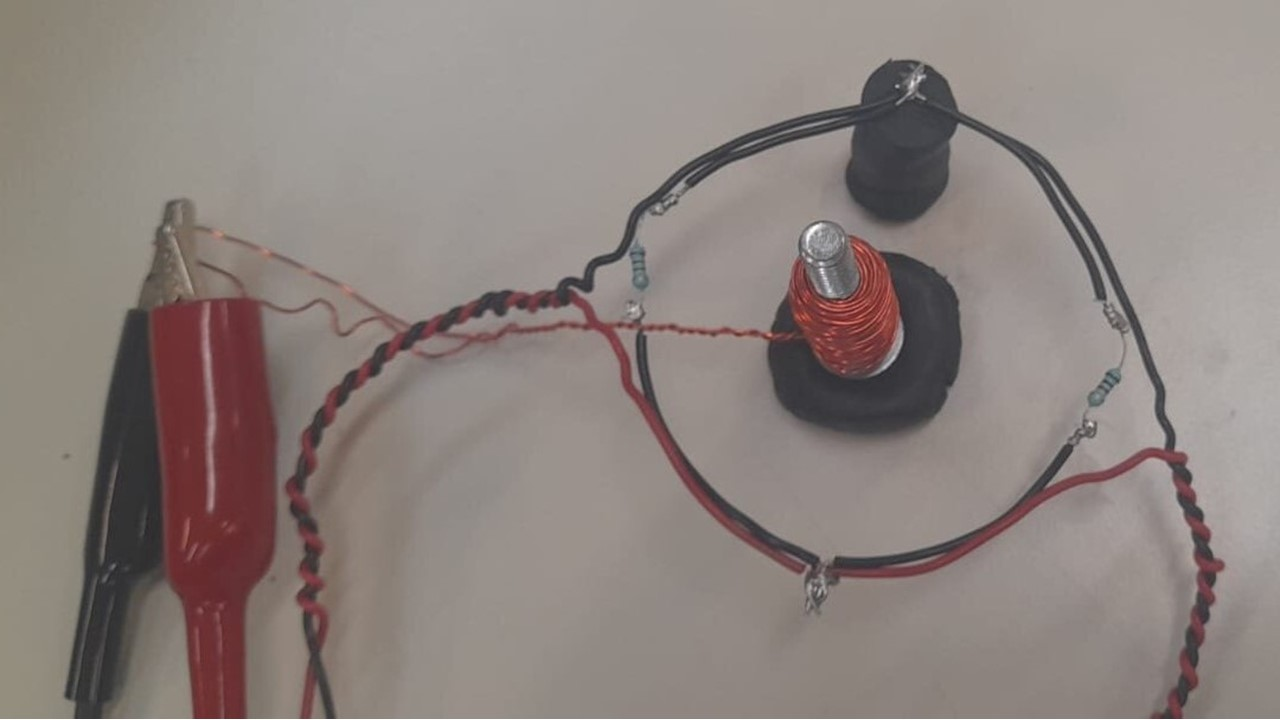
\includegraphics[scale=0.5]{Circuito2.jpg}
    \captionof{figure}{ Representación física del circuito}
\end{center}\vspace{0.4cm} 


\noindent Se usó una fuente de 22 V que sería conectada al solenoide. Las resistencias usadas tienen valores de $1k\Omega$ y $2.2k\Omega$.

\vspace{0.3cm}
Para hacer una aproximación práctica al flujo magnético que fue propuesto al inicio, lo que se hizo fue conectar y desconectar la fuente de voltaje de manera repetitiva y capturar las mediciones durante el momento que cambia el flujo a través de la espira.

Se utilizó un osciloscopio \textit{Agilent Technologies DSO1002A}, que se le conectaron las dos puntas  de medición, a las cuales se les aplicó un escalamiento digital X$10$ de las señales medidas.
\section*{Resultados}
\noindent Ahora mostraremos los resultados obtenidos de los "potenciales" medidos con un osciloscopio en los mismos puntos:  
 
\begin{center}\vspace{0.4cm}
    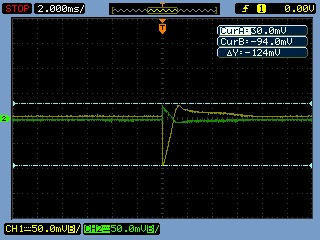
\includegraphics[scale=1.5]{Circuito3.jpeg}
    \captionof{figure}{ Captura del osciloscopio}
\end{center}\vspace{0.4cm}

\noindent Como puede apreciarse en la $\textbf{Fig. 3}$, la señal de color verde que corresponde a la punta conectada a la resistencia de \textit{1.1$ K\Omega$} con una lectura de \textit{30 mV} y la amarilla que corresponde a una de \textit{2.2$K \Omega$} con una lectura de \textit{-94 mV}. Podemos apreciar lo mencionado con los cálculos realizados previamente de los cuales notábamos que $V_{1}$ y $V_{2}$ siempre serían de signos opuestos.

Sin embargo, tenemos un error sistemático que no nos permitió corroborar de manera cuantitativa la ecuación \ref{corriente2}, tomando en cuenta un error del 5$\%$ sobre el valor de las resistencias donde para la resistencia de \textit{1.1$K \Omega$} se calculó una corriente de \textit{[3 $\pm$ 0.15]$\cdot 10^{-5}$A }, y para la de \textit{2.2$K \Omega$} una de \textit{[4.25 $\pm$ 0.25]$\cdot 10^{-5}$ A}

%----------------------------------------------------------------------------------------
%	CONCLUSIONS
%----------------------------------------------------------------------------------------

\color{Black} % SaddleBrown color for the conclusions to make them stand out

\section*{Conclusiones}

\noindent Los datos experimentales concuerdan de manera cualitativa con la teoría que previamente realizamos, que es justamente como esperábamos. Entonces el problema planteado al comienzo, donde nos cuestionábamos qué pasaría con las mediciones, de ahí podemos afirmar que los "potenciales" medidos  fueron distintos aun midiendo en los mismos puntos, lo que nos indica que el  $\nabla \times \text{E}$ debe ser distinto de cero y por consecuencia tenemos un campo no conservativo, en los cuales  \textbf{ se debe tener a consideración la geometría y topología de la situación física} ya que se presentan resultados que no son evidentes y podemos decir que van en contra de la intuición.

\color{Black} % Set the color back to DarkSlateGray for the rest of the content

%----------------------------------------------------------------------------------------
%	REFERENCES
%----------------------------------------------------------------------------------------

\section*{Referencias}

\textbf{[1]}
Romer, R. H. (1982). What do ‘“voltmeters”’ measure?: Faraday’s law in a multiply connected region. American journal of physics, 50(12), 1089–1093. https://doi.org/10.1119/1.12923
\vspace{0.4cm}

\textbf{[2]} Griffiths, D. (2017). Introduction to Electrodynamics (4th ed.). Cambridge: Cambridge University Press. doi:10.1017/9781108333511


\end{multicols}
\end{document}